% A parabola with the tangent line at (p, f(p)) in red and the secant
% line through (p+h, f(p+h)) dashed in green, illustrating the derivative
% as the limiting slope of secants.
% Source: book/tex/calculus/differentiate.tex (§ Definition of derivative).
\documentclass[border=2mm]{standalone}
\usepackage{tikz}
\begin{document}
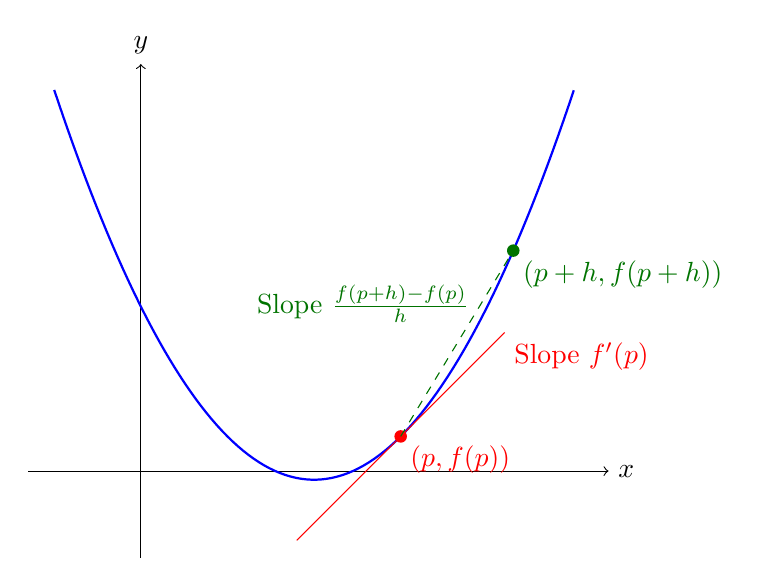
\begin{tikzpicture}[scale=1.1,
    dot/.style={circle,fill,inner sep=1.6pt}]
  \draw[->] (-1.3,0)--(5.4,0) node[right] {$x$};
  \draw[->] (0,-1)--(0,4.7) node[above] {$y$};
  \draw[blue,thick,domain=-1:5,samples=100]
    plot (\x, {(\x-2)*(\x-2)/2-0.1});
  % point (p,f(p)) at p=3, f=0.4
  \node[dot,red] at (3,0.4) {};
  \node[red,below right] at (3,0.4) {$(p,f(p))$};
  % tangent line at p=3 (slope 1)
  \draw[red] (1.8,-0.8)--(4.2,1.6);
  \node[red,below right] at (4.2,1.6) {Slope $f'(p)$};
  % point (p+h, f(p+h)) at 4.3, f=2.545
  \node[dot,green!45!black] at (4.3,2.545) {};
  \node[green!45!black,below right] at (4.3,2.545) {$(p+h,f(p+h))$};
  % secant
  \draw[green!45!black,dashed] (3,0.4)--(4.3,2.545);
  \node[green!45!black,above left] at (3.9,1.6)
    {Slope $\frac{f(p+h)-f(p)}{h}$};
\end{tikzpicture}
\end{document}
